% Created 2021-04-19 Mon 19:27
% Intended LaTeX compiler: pdflatex
\documentclass[11pt]{article}
\usepackage[utf8]{inputenc}
\usepackage[T1]{fontenc}
\usepackage{graphicx}
\usepackage{grffile}
\usepackage{longtable}
\usepackage{wrapfig}
\usepackage{rotating}
\usepackage[normalem]{ulem}
\usepackage{amsmath}
\usepackage{textcomp}
\usepackage{amssymb}
\usepackage{capt-of}
\usepackage{hyperref}
\usepackage[utf8]{inputenc}
\usepackage[english]{babel}
\setlength{\parindent}{4em}
\setlength{\parskip}{1em}
\renewcommand{\baselinestretch}{2.0}
\author{Daniel Zehr, Inaara Sarfani, Matthew Cuong Lam, Tanya Panesar, \& Umeira Vijendra}
\date{\today}
\title{PSYCH 363 - Implicit Association Test: Self-Esteem}
\hypersetup{
 pdfauthor={Daniel Zehr, Inaara Sarfani, Matthew Cuong Lam, Tanya Panesar, \& Umeira Vijendra},
 pdftitle={PSYCH 363 - Implicit Association Test: Self-Esteem},
 pdfkeywords={},
 pdfsubject={},
 pdfcreator={Emacs 26.3 (Org mode 9.1.9)}, 
 pdflang={English}}
\begin{document}

\maketitle
\tableofcontents




\section{Introduction}
\label{sec:org0588127}


The use of experimental tests have been employed in Psychology ever since it was born. Ever since then there has been the development of a number of psychological tests to measure certain variables. One particular test that has been developed uses implicit attitudes to measure a person's underlying automatic evalutation on a certain subject, this is known as the Implicit Association Test (IAT) \cite{greenwald_mcghee_schwartz_1998}. This test works by displaying target words or images on screen and having participants respond to pairs of attitude objects (e.g. self vs other) or affective concepts (e.g. positive vs negative) by pressing a left versus right response key. The reaction time to attribute the response to the target object is then taken as an indicator of implicit attitudes. Past researchers have used this method to test a variety of implicit attitudes, such as attitudes towards one parent \cite{Yang_2013} or the subjective well-being of oneself \cite{Walker_Schimmack_2008}. More notably IAT measures are often used as self-esteem measures using words to describe a person's chracteristic and measuring how fast one responds to characteristics that they might attribute to themself. Taking inspiration from the study done by Karpinski (2004) we will adopt a similar format using a word bank of describing characterisitcs to measure implicit attitudes towards self-esteem. 

\section{Method}
\label{sec:org6c47a12}

\textbf{Subjects}

Students from group 3 of Computing and Psychological Research course at University of Waterloo and their respective family members and friends participated in the study. The study consists of 8 subjects in total. 

\noindent
\textbf{Procedure}

In the IAT, the subject responds to a series of items that are to be classified in 2 categories, one assessing the associations of self versus other and the other representing an attribute discrimination such as pleasant versus unpleasant words. The experiment consisted of 5 blocks of categorization trials. In each step, the subject presses a left or right key to categorize each stimuli which are presented on the desktop screen. The computer recorded the elapsed time between the beginning presentation of each stimulus and occurrence of keyboard response of block 3 and block 5.

Part 1 consists of instructions for the subject to understand what is needed from them. In the first step, the subjects practice a target concept by classifying items into self and other categories. The second step includes categorizing pleasant and unpleasant words. In the third step, the subject groups items into 2 integrated categories, ie, it includes the target and attribute concept, assigned to the same key in the previous two steps. For instance, self+pleasant (left key), other+unpleasant(right key). The fourth step is the practice test with reverse keys for either the target or attribute concept. The last step involves a switched key experiment. For example, self+unpleasant (left key) or other+pleasant(right key). 

\section{Results}
\label{sec:orgb7e5296}


Analyses focus on participants' keyboard response times to both positive and negative words presented in the third and fifth block trials of the experiment, where the response keys were switched.


A slight variation among response times exists between participants’ responses to positive versus negative words, in that, negative words incurred a slightly longer average, standard deviation, and median keyboard response time across both conditions (Table 1). 

\noindent
\textbf{Table 1}
Descriptives of Reaction Times 

\begin{verbatim}
                    Mean        SD    Median
Positive Words 0.8545347 0.3109061 0.7911803
Negative Words 0.9436601 0.3209012 0.9436601
\end{verbatim}

\noindent
\textbf{T-Tests}

Two t-tests were conducted to compare reaction times with positive and negative words among the two conditions. There was not a significant relationship in reaction times for positive words when it was paired with either self or other (blocks 3 and 5 respectively), \emph{t} (7) =  , \emph{p} > 0.05, \emph{d} = . This  was also found with the negaitve words as there was a  non-significant relationship between the two blocks, \emph{t} (7) = -1.3768, \emph{p} > 0.05, block 5 \emph{t} (7) = -0.23742, \emph{p} > 0.05, \emph{d} = .   

\newpage

\noindent
\textbf{Figure 1: Negative and Positive Reaction Times in both trial blocks}
\begin{center}
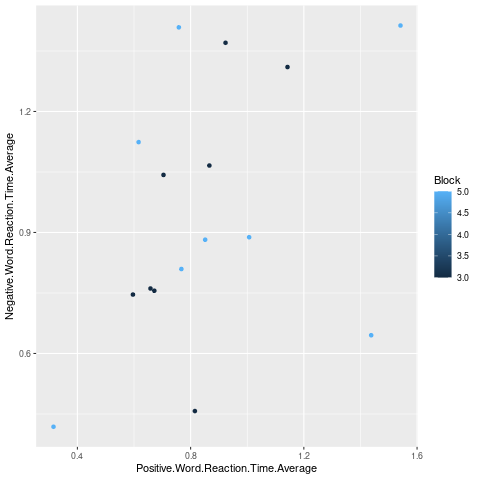
\includegraphics[width=.9\linewidth]{plot.png}
\end{center}

On observation of the negative and positive word reaction times for each comparative trial block 
no significant difference is evident. Despite this result, the plot seems to show a similar pattern as Table 1 with an overall decrease in average reaction times for positive words in comparison to negative words regardless of condition, although it should be noted that this relationship is non-significant (Figure 1). 

\section{Discussion}
\label{sec:org1c8c48f}


The experiment examines the elapsed time of each stimulus and the reaction time which consists of 16 observations of 8 variables (steps 3 and 5). 
The insignificance for both T-tests is expected as the sample size is small in comparison to past research \cite{greenwald_farnham_2000}. It was hypothesized that individuals will respond much faster to positive items about self. Our results showed a slightly higher mean for negative reaction time average (0.94366 sec) than positive time average (0.8545 sec), suggesting that participants responded to positive items faster than negative. Furthermore, the average number of correct keystrokes for positive and negative words are the same (26) and indicates that participants were equally likely to refer to themselves with positive words as to others for negative. Using this information we could compare results with an explicit self-esteem test to observe any differences or similarities between words that participants positively associate themselves with  \cite{greenwald_farnham_2000}. It would be expected that those with a higher self-esteem would react quicker to positive words that are associated with themselves compared to those with low self-esteem. In our experiment we observed a slightly faster reaction time to positive words than negative words which follows the trends of previous research. With a larger sample a more definitive result could be reached. 
\newpage

\addcontentsline{toc}{section}{References}
\bibliographystyle{apalike}
\bibliography{references}
\end{document}
